\chapter{Implementierung}
Nach dem Entwurf des Systems wurde mit der Implementierung begonnen.
Hierbei wurde zuerst das \acs{FPGA}-Design umgesetzt und anschließend durch Simulation verifiziert.

Nachfolgend wurde mit der Erstellung des \acs{PYNQ}-Images begonnen und erst abschließend wurde die Python-Software(Notebooks) zur Systemsteuerung umgesetzt.
Final erfolgte ein Test des Gesamtsystems durch Empfang eines, durch einen Funktionsgenerator erzeugten, Testsignales.

Die folgenden Abschnitte sollen detailliert den verwendeten Entwicklungsprozess sowie das vorgehen bei der Implementierung der einzelnen Komponenten beschreiben.

\clearpage
\section{FPGA-Design} \label{Chap:Impl}
Die Erstellung des \acs{FPGA}-Designs erfolgte in der Hardwarebeschreibungssprache \acs{VHDL}. Diese wurde aufgrund von bestehender Erfahrungen und der bekannten Syntax ausgewählt.

Als Entwicklungsumgebung für die in \acs{VHDL} geschriebenen Komponenten wurde die \textbf{Sigasi IDE}\footnote{\href{https://www.sigasi.com}{https://www.sigasi.com}} verwendet.
Hierbei handelt es sich um eine Eclipse basierte Entwicklungsumgebung, die sich (im Vergleich zu Proprietären \acs{FPGA}-Entwicklungsumgebungen) besonders durch ihre einfache Bedienung und eine schnelle Reaktionszeit auszeichnet.
\begin{figure}[h]
	\centering
	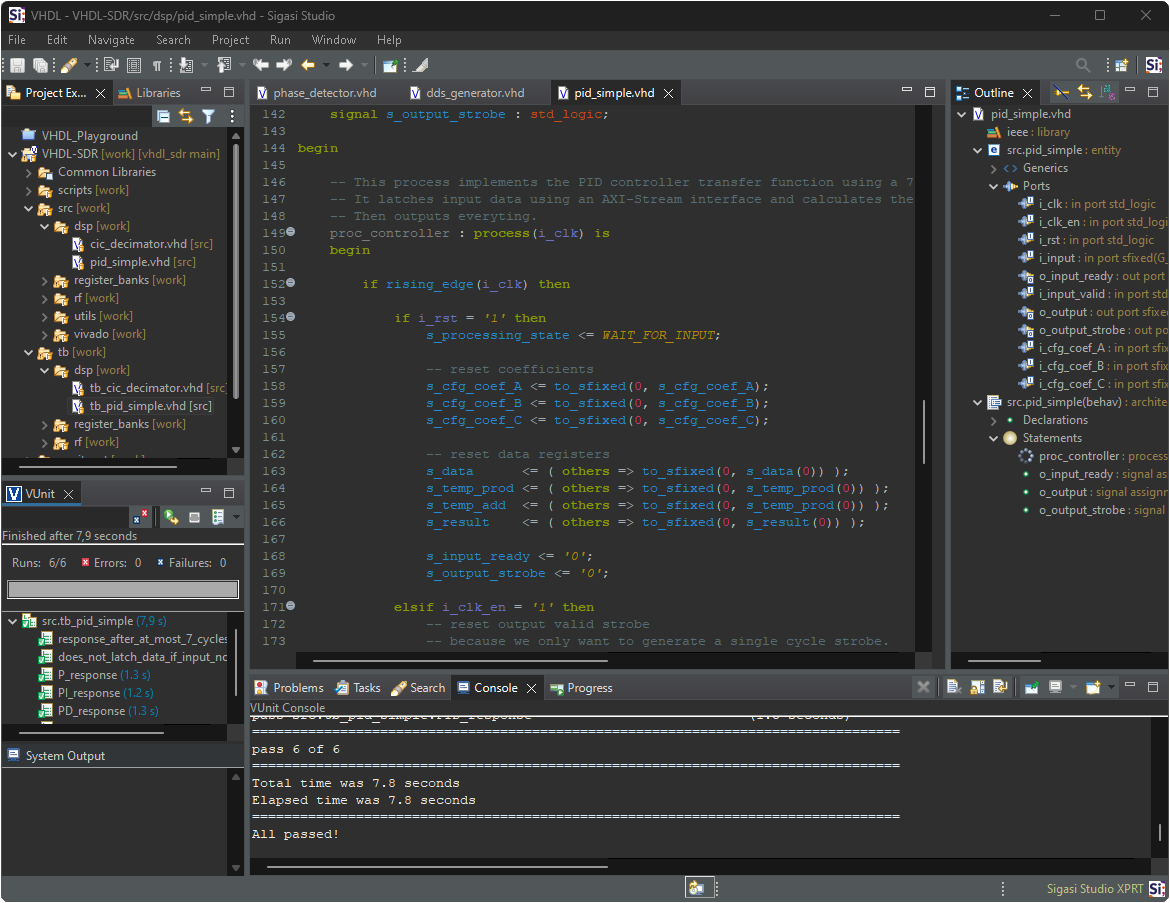
\includegraphics[width=\linewidth]{Sigasi}
	\caption{Screenshot der Sigasi IDE}
\end{figure}

Besonders Komfortabel an dieser Entwicklungsumgebung, ist die Möglichkeit externe Simulatoren (z.B. XSIM oder GHDL) sowie externe Testframeworks (z.B. OSVVM, VUnit) 
einfach integrieren zu können und so Tests direkt aus der Entwicklungsumgebung möglich machen.

Als Verifikationsframework wurde \textbf{VUnit}\footnote{\href{https://vunit.github.io}{https://vunit.github.io}} verwendet.
Hierbei handelt es sich um Open-Source Unit-Testing Framework für VHDL welches über Python angesteuert werden kann und bereits viele Verfikationskomponenten (z.B. Bus-Master) beinhaltet.

Als besonders nützlich stellte sich hier die Möglichkeit Python für die Erstellung und Verifikation von Testdaten nutzen zu können heraus.
Das hierzu angewendeten Verfahren wird näher bei der Verifikation der einzelnen Komponenten beschrieben. 

Als Simulator wurde \textbf{GHDL}\footnote{\href{http://ghdl.free.fr}{http://ghdl.free.fr}} verwendet.

Für die Synthese und OnChip-Implementierung des Designs sowie die Erstellung des Block-Designs des \acs{FPGA}-Bitstreams wurde die von Xilinx bereitgestellte Entwicklungsumgebung \textbf{Vivado} verwendet.

\subsection{Vorgehen bei der Implementierung}

Begonnen wurde die Implementierung mit der Erstellung des \acs{VHDL}-Codes.

\begin{figure}[h]
	\centering
	\begin{tikzpicture}[scale=0.85, every node/.style={scale=0.85}, node distance=2cm]
		
		\tikzstyle{startstop} = [rectangle, rounded corners, minimum width=3cm, minimum height=1cm,text centered, draw=black, fill=red!30]
		\tikzstyle{process} = [rectangle, minimum width=4.5cm, minimum height=1cm, text centered, draw=black, fill=orange!30]
		\tikzstyle{decision} = [diamond, minimum width=3cm, minimum height=1cm, text centered, draw=black, fill=green!30]
		\tikzstyle{arrow} = [thick,->,>=stealth]

		\node (start) [startstop] {Start};
		\node (impl) [process, below of=start] {Implementierung};
		\node (sim) [process, below of=impl] {Simulation};
		\node (sim_ok) [decision, below of=sim]  {OK?};

		\node (synth) [process, below of=sim_ok] {Synthese};
		\node (timing) [process, below of=synth] {Check Timing};
		\node (timing_ok) [decision, below of=timing]  {OK?};
		\node (schem) [process, below of=timing_ok] {Check Schematic};
		\node (schem_ok) [decision, below of=schem]  {OK?};
		\node (docu) [process, below of=schem_ok]  {Dokumentation};
		\node (stop) [startstop, below of=docu] {Fertig};
		
		\draw [arrow] (start) -- (impl);
		\draw [arrow] (impl) -- (sim);
		
		\draw [arrow] (sim) -- (sim_ok);
		\draw [arrow] (sim_ok.east) -- ++(2,0) node[midway, anchor=south]{Nein} |- (impl.-5);
		\draw [arrow] (sim_ok.south) -- (synth) node[midway, anchor=west]{Ja};
		
		\draw [arrow] (synth) -- (timing);
		\draw [arrow] (timing) -- (timing_ok);
		\draw [arrow] (timing_ok.east) -- ++(2.5,0) node[midway, anchor=south]{Nein} |- (impl.east);
		\draw [arrow] (timing_ok.south) -- (schem) node[midway, anchor=west]{Ja};
		
		\draw [arrow] (schem) -- (schem_ok);
		\draw [arrow] (schem_ok.east) -- ++(3,0) node[midway, anchor=south]{Nein} |- (impl.5);
		\draw [arrow] (schem_ok.south) -- (docu) node[midway, anchor=west]{Ja};

		\draw [arrow] (docu) -- (stop);

	\end{tikzpicture}
	
	\caption{Ablauf der Implementierung} \label{Abb:Impl}
\end{figure}
 
Hierbei wurden zuerst die Eingangs-/Ausgangsports der einzelnen Komponenten spezifiziert. 
Anschließend wurde die im Entwurf festgelegte Funktionalität umgesetzt. 

Wo möglich wurden funktional zusammengehörige Gruppen in eigene Komponenten ausgelagert, diese dann separat umgesetzt und dabei möglichst generisch gestaltet.

Besonderes Augenmerk lag ebenfalls auf dem effizienten Mapping von \acs{VHDL}-Code auf die einzelnen primitiven Logikelementen welche der \acs{FPGA} zur Verfügung stellt.. 
So wurde z.B. besonders Multiplikationen so umgesetzt, dass bei der späteren Synthese möglichst viele vorhandene \acs{DSP}-Slices bei der Synthese verwendet werden können.
Besonders hilfreich war hier die von Xilinx zur Verfügung gestellte Dokumentation zum Aufbau der vorhanden DSP-Slices\cite{XLX_DSP}.

Nach bzw. während der Erstellung des \acs{VHDL}-Codes wurde eine funktionelle Simulation der einzelnen Komponenten durchgeführt.
Hierbei wurden Testfälle (Testbenches) erstellt welche, soweit möglich, die Funktionalität der Komponenten bereits selbstständig verifizieren.
Dies sollte den manuelle Verifikationsaufwand gering halten und die Wiederholbarkeit der Testfälle erhöhen.
Besonders vereinfacht wurde die Testfallerstellung durch die von VUnit bereitgestellten Bibliotheken sowie der Möglichkeit externe Python-Scripte in den Testfällen zu verwenden.
Wo eine automatische Testfallüberprüfung nicht möglich wurde das Verhalten der Komponenten manuell überprüft.

Nach Durchführung der Simulation wurden die einzelnen Komponenten separat in Vivado synthetisiert.
Anhand diesen synthetisierten Designs wurden anschließend das Erreichen der gewünschten maximalen Taktrate überprüft.
Wurde diese initial nicht erreicht so wurde der \acs{VHDL}-Code durch Einführung von Zwischenregistern (Pipelining) angepasst, bis die gewünschte Taktrate erreicht wurde.

Besonders wichtig, wenn auch mühselig, war hier ebenfalls die Kontrolle des von Vivado erstellten Schaltplanes um zu überprüfen ob die gewünschten Hardware-primitiven (z.B. \acs{DSP}-slices)
richtig eingefügt werden konnten. 
Hilfreich waren hier besonders die von Vivado bereitgestellten Build-Logs aus welchen Informationen zu verwendeten primitiven gewonnen werden konnten (DSP-Utilization-Report).

Nach funktionaler Fertigstellung des \acs{VHDL}-Codes wurde abschießend Dokumentation erstellt welche die einzelnen Komponenten sowie deren interne Funktion beschreiben und erklären soll.
Die Dokumentation wurde in der Form von Inline-Code-Dokumentation erstellt.

Der hier beschriebenen Implementierungsprozess wird ebenfalls von \ref{Abb:Impl} dargestellt.

\clearpage

\subsection{Mischer (Mixer)}
Der Mischer hat die Aufgabe den vom \acs{ADC} gewonnenen Datenstrom mit den vom \acs{NCO} erzeugten Trägersignalen zu Multiplizieren.
Aufgrund der Tatsache, dass dies vor der Dezimierung des Eingangssignals erfolgt, handelt es sich hier um eine kritische Stelle. 
Deren Performance die maximale Taktrate bestimmt, mit dem das System betrieben werden kann.

Es wurde deswegen besonders darauf geachtet, den \acs{VHDL}-Code so zu gestalten, dass für die notwendigen Multiplikationen \acs{DSP}-Slices verwendet werden können.

Die Multiplikationsoperanden sowie das Ergebnis werden im Festkomma-Format dargestellt.
Das Ergebnis der Multiplikation wird auf die Bit-Breite des Eingangssignales gerundet. Die Rundungsart ist einstellbar. 

\subsection{Lokaler Oszillator (NCO)}
Die Umsetzung des lokalen Oszillators erfolgt anhand der in \ref{Sec:NCO} beschriebenen Struktur.
Da hier ebenfalls einmal pro \acs{ADC}-Taktzyklus Ausgangswerte generiert werden müssen, handelt es sich hier ebenfalls um ein Performance-kritisches Modul.

Es wurde deswegen besonders drauf geachtet, die notwendigen Sinus/Kosinus Lookup-Tabellen als Block-RAM (\acs{BRAM}) umsetzen zu können.

Für langsame Trägersignale wurde hier zusätzlich die (optionale) Möglichkeit geschaffen zwischen Stützstellen der Lookup-Tabelle linear zu interpolieren.
Diese Option bietet besonders bei geringen Trägerfrequenzen und einer geringen Anzahl von Stützstellen einen Gewinn in der Güte des Trägersignales.
Dies erfolgt jedoch auf Kosten der maximalen erreichbaren Taktfrequenzen.

Zusätzlich kann jeder Träger optional invertiert werden um etwaige Vorzeichenprobleme im Empfänger auszugleichen.

Nach \cite{IEEE_ART_DDS} wären mehrere Maßnahmen denkbar, welche die Größe der Lookup-Tabelle verringern ohne die Anzahl der Stützpunkte zu reduzieren.
Aus Einfachheit wurde hier jedoch drauf verzichtet und der Oszillator verwendet eine Lookup-Tabelle deren Größe der Anzahl der Stützpunkte entspricht.

Die unterschiedlichen Parameter des Oszillators (Akkumulatorbreite $n$, Anzahl der Stützstellen $2^m$, sowie die Bitbreite der erzeugten Träger kann über generische
Parameter während der Synthese eingestellt werden.

Die Verifikation des Oszillators erfolgte durch eine spektrale Analyse der erzeugten Träger.
Anhand des ermittelten Spektrums der erzeugten Träger wurden Position der Grundschwingung, Anteil und Amplitude der Harmonischen und die Phasenlage der Träger zueinander ermittelt.
Dies erfolgte für unterschiedliche Parameterkonfigurationen.

Die folgende Abbildung \ref{Abb:Carrier} zeigt beispielhaft das Spektrum eines erzeugten Kosinus-Trägers für eine Oszillatorfrequenz $f=\qty{14.41}{M\hertz}$ bei einer \acs{ADC}-Taktrate von $f_{ADC}=\qty{100}{M\hertz}$ einer 
Akkumulatorbreite von $n=\qty{21}{bit}$ und einer Anzahl von $1024$ Stützpunkten ($m=\qty{10}{bit}$)

\begin{figure}[h]
	\centering
	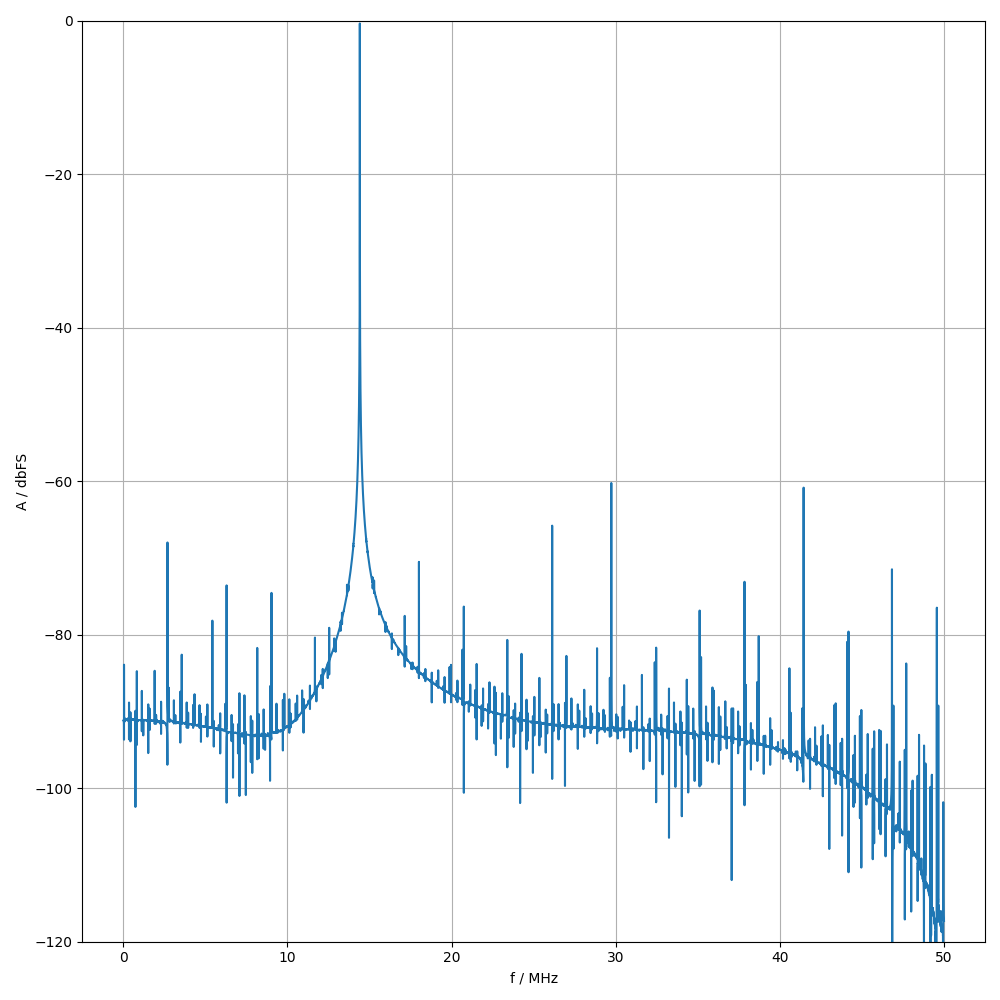
\includegraphics[width=0.8\linewidth]{spectrum_cos}
	\caption{Spektrum des $cos$ Trägers für: $f_{adc}=\qty{100}{M\hertz},f=\qty{14.41}{M\hertz}, n=21, m=10$ }
	 \label{Abb:Carrier}
\end{figure}

Die aus der Theorie erwarteten Kenngrößen\cite{IEEE_ART_DDS} konnten durch die gemessen Daten bestätigt werden.

\subsection{\acs{CIC}-Dezimerungssfilter}
Die Implementierung des \acs{CIC}-Dezimierungssfilter wurde anhand des in \ref{Sec:CIC} spezifizierten Entwurfs durchgeführt.

Soweit möglich können die Filterparameter (Ordnung $N$, Dezimierungsrate $R$) über generische Parameter während der Synthese festgelegt werden.

Um die Implementierung des Filters zu vereinfachen wurde hier jedoch bestimmte Einschränkungen der Parameter getroffen:
\begin{itemize}
	\item der Dezimierungsfaktor muss eine Zweierpotenz sein\\
	      \textit{(Dies vereinfacht die Normalisierung des Filter-Gains, da die Division durch Potenzen von Zwei durch Routing erfolgen kann)}
	\item die Filterordnung muss größer oder gleich dem Dezimierungsfaktor sein\\
		  \textit{(Notwendig um die Differenzierer, sequenziell und ohne Pipelining, umsetzen zu können)} 
\end{itemize}

Da der \acs{CIC}-Filter, vor der Dezimierung, ebenfalls Daten mit dem \acs{ADC}-Taktfrequenz verarbeitet, handelt es sich hier ebenfalls um eine Komponente mit kritischen Pfaden.
Optimierungspotential wäre hier, durch Flexibilisierung der intern verwendeten Bit-Breiten (pruned-\acs{CIC}-Filter) und folglicher Reduktion der Schaltungskomplexität, noch vorhanden.

Die Verifikation des Filters erfolgte durch Vergleich der Sprungantwort mit einer von Matlab erzeugten Referenzkurve.

\subsection{Phasen-Komparator}
Der Phasen-Komparator ermittelt anhand der im Entwurf (vergleiche \ref{Sec:PD}) beschriebenen Gleichungen die Phasenabweichung des Eingangssignals.

Da der Phasen-Komparator bereits mit dem dezimierten Eingangssignal arbeitet sind hier mehrere Taktzyklen für die Verarbeitung des Datenwerts vorhanden.
Die Durchführung der Berechnung wurde deswegen in der Form eines Zustandsautomates umgesetzt.

\begin{figure}[h]
	\centering
	\begin{circuitikz}[scale=0.7, every node/.style={scale=0.7}]
		\tikzset{flipflop DE/.style={flipflop, flipflop def={t1=D, td=EN, t6=Q, c3=1, t4=\ctikztextnot{Q}}}}
		\tikzset{
			LUT/.style={muxdemux, muxdemux def={Lh=4, Rh=4, w=5, NB=0, NR=1, NL=2}, muxdemux label={L1=A, L2=B, R1=C}},
			CTRL/.style={muxdemux, muxdemux def={Lh=4, Rh=4, w=5, NB=0, NR=1, NL=2, NT=3}, muxdemux label={L1=In\_Valid, L2=Clock, cL2=1, R1=Out\_Valid, T1=EN0, T2=EN1, T3=EN3}}
		}	
		\tikzset{
			basic/.style={rectangle,draw=black, top color=white,text centered},
			branch/.style={fill,circle,minimum size=5pt,inner sep=0pt,outer sep=-1pt},
    		buswidth/.style={decoration={ markings,
  				mark= at position 0.0 with {\node[font=\footnotesize] {/};\node[below=1pt] {\tiny #1};}
  			}, postaction={decorate}}
 		}	
		
		% Input buffer registers
		\node[flipflop DE] (REG_Q) at (0,0) {REG\_Q};
		\node[flipflop DE] (REG_I) at (0,3.5) {REG\_I};

		% Mutiply
		\node[LUT, muxdemux label={N=OP\_MUL\_Q}] (OP_Q) at (5,0) {$B\cdot sign(A)$};
		\node[LUT, muxdemux label={N=OP\_MIL\_I}] (OP_I) at (5,3.5) {$A\cdot sign(B)$};

		% Temporary Storage Registers
		\node[flipflop DE] (REG_TQ) at (9,0) {REG\_TQ};
		\node[flipflop DE] (REG_TI) at (9,3.5) {REG\_TI};

		% Adder
		\node[LUT,muxdemux label={N=OP\_ADD}] (OP_ADD) at (13,2.0) {$B - A$};


		% Output register
		\node[flipflop DE] (REG_OUT) at (17,2) {REG\_O};

		% Control block
		\node[CTRL] (CTRL) at (5,-3.5) {\acs{FSM}};

		% Inputs		
		\draw[buswidth=n] (REG_I.pin 1) -- ++(-2,0) node[left]{IN\_I};
		\draw[buswidth=n] (REG_Q.pin 1) -- ++(-2,0) node[left]{IN\_Q};

		% Input buffer to Multiply
		\draw[buswidth=n] (REG_I.pin 6) -- ++(1.5,0) node[branch](bI0){};
		\draw (bI0) -| (OP_I.lpin 1);
		\draw (bI0) |- (OP_Q.lpin 1);
		
		\draw[buswidth=n] (REG_Q.pin 6) -- ++(0.75,0) node[branch](bQ0){};
		\draw (bQ0) |- (OP_I.lpin 2);
		\draw (bQ0) |- (OP_Q.lpin 2);

		% Mutiply to Temp buffer
		\draw[buswidth=n] (OP_I.rpin 1) -| (REG_TI.pin 1);
		\draw[buswidth=n] (OP_Q.rpin 1) -| (REG_TQ.pin 1);

		% Temp Buffer to adder
		\draw[buswidth=n] (REG_TI.pin 6) -| (OP_ADD.lpin 1);
		\draw[buswidth=n] (REG_TQ.pin 6) -| (OP_ADD.lpin 2);

		% adder to output register
		\draw[buswidth=n] (OP_ADD.rpin 1) -| (REG_OUT.pin 1);

		% output
		\draw[buswidth=n] (REG_OUT.pin 6) -- ++(1,0) node[right]{$e_\varphi$};

		% Clock enable, Input
		\draw (REG_I.down) -| ++(-1.3,-3.5) node[branch](clkEnB0){};	
		\draw (clkEnB0) -- (REG_Q.down);
		\draw (clkEnB0) |- (CTRL.tpin 1);	
		
		\draw (REG_TI.down) -| ++(-1.3,-3.5) node[branch](clkEnB1){};	
		\draw (clkEnB1) -- (REG_TQ.down);
		\draw (clkEnB1) -| (CTRL.tpin 2);	
		
		\draw (CTRL.tpin 3) -| (REG_OUT.down);	

		% Input valid
		\draw (CTRL.lpin 1) -- ++(-6.5,0) node[left]{IN\_Valid};		
		
		% Output valid
		\draw (CTRL.rpin 1) -- ++(11,0) node[right]{OUT\_Valid};	
		
		% Clock
		\draw (REG_I.pin 3) -| ++(-0.75,-3.5) node[branch](clkB0){};	
		\draw (clkB0) -- (REG_Q.pin 3);		
		\draw (clkB0) -- ++(0,-4.5) node[branch](clkB1){};
		\draw (clkB1) -- ++(-1.4,0) node[left]{Clock};
		\draw (clkB1) -- ++(9,0) node[branch](clkB2){};
		\draw (clkB2) -- ++(0,4.5) node[branch](clkB3){};
		\draw (clkB3) -- (REG_TQ.pin 3);
		\draw (clkB3) |- (REG_TI.pin 3);
		\draw (clkB2) -- ++(5,0) node(clkB3){};
		\draw (clkB3.west) -| (REG_OUT.pin 3);
		\draw (CTRL.lpin 2) -| ++(-1,-1.255) node[branch]{};	
		
	\end{circuitikz}
	\caption{Vereinfachter Schaltplan des Phasen-Komparators.}
\end{figure}

Ein Zustandsautomat übernimmt hier die Erzeugung der Clock-Enable Signale welche den Datenfluss durch das Modul steuern.
Die explizite Datenflusssteuerung ist notwendig, da nicht jeden Taktzyklus gültige Daten am Eingang empfangenen werden.
Da die Ermittlung des Phasenfehlers bereits mit reduzierter Datenrate erfolgt, ist es darüber hinaus nicht notwendig jeden Taktzyklus einen Wert verarbeiten zu können.

Zwischen zwei Registern befindet sich die kombinatorische Logik welche die notwendigen arithmetischen Operationen umsetzt und so die eigentliche Datenverarbeitung übernimmt.

Die Umschaltung zwischen den Modulationsarten, im obigen Schaltplan aus Übersichtlichkeitsgründen nicht enthalten, erfolgt durch Anpassung der Differenzbildung
im Block \lstinline|OP_ADD|, für \acs{BPSK}: $C = B$, für \acs{QPSK}: $C=B-A$.

\subsection{\acs{PID}-Regler}
Der \acs{PID}-Regler implementiert die in Absatz \ref{Sec:PID} ermittelte Übertragungsfunktion.

Die Umsetzung erfolgt hier, ähnlich wie bei dem Phasen-Komparator, wieder anhand eines Zustandsautomaten der die einzelnen Rechenoperationen sequenziell abarbeitet.

Es werden dadurch mehrere Taktzyklen für die Verarbeitung eines Eingangswertes benötigt.
Da der \acs{PID}-Regler jedoch ebenfalls bereits dezimierte Signale verarbeitet stehen diese Taktzyklen zur Verfügung. 

Die einzelnen für die Berechnung notwendigen Rechenschritten wurden so umgesetzt, mit so eventuell notwendigen Wartezyklen, so das möglichst viele Operation (Multiplikationen/Additionen) in 
\acs{DSP}-Slices verlagert werden können. So ist lediglich ein mit Logikelementen umgesetzter Addierer für das Endergebnis nötig.

Die Berechnung der Reglerantwort wird intern jeweils in Festkommadarstellung und mit voller Genauigkeit durchgeführt.
Am Ende der Berechnung erfolgt eine einzelne Rundung auf das Ausgangsformat. Die Rundungsart (Runden,Abscheiden) ist hierbei einstellbar.

Die Verifikation erfolgte durch Überprüfung der Sprungantwort für unterschiedliche Werte der Reglerparameter $A,B$ und $C$.
Die hierzu verwendete Referenzsprungantwort wurde mit Matlab erzeugt.

\subsection{RF-Reciever}
Der RF-Reciever bildet das Top-Level Modul des in \acs{VHDL} erstellten Teils des \acs{FPGA}-Designs.

der RF-Reciever verschaltet Mischer, den lokalen Oszillator, die \acs{CIC}-Dezimierungsfilter für $I$ und $Q$ Datenpfad, 
den Phasen-Komparator und den \acs{PID}-Regler zu einer Phasen-Regelschleife welche die Demodulation des Eingangssignales inklusive Trägerrekonstruktion übernimmt.

Grundsätzlich erfolgt hier größtenteils nur eine Instanziierung der bereits erstellten Komponenten.
Lediglich kleinere Logikteile, welche benötigt werden um die Komponenten verschalten zu können, sind hier umgesetzt.

So ist z.B. zwischen lokalem Oszillator und \acs{PID}-Regler ein Register notwendig, welches die \acs{AXI}-Stream Schnittstelle am Ausgang des \acs{PID}-Reglers 
auf den direkten Logikeingang des Oszillators anpasst.

Zusätzlich wurde der gesamte Empfangsteil anschließend, für unterschiedlichen Parameter (Trägerfrequenzen, Signal/Rauschverhältnis), durch Simulation getestet.
Es wurde zusätzlich die empirische Einstellung des Reglers vorgenommen.

Bei der Simulation wurden, mit Python, jeweils ein modulierter Datenstrom erzeugt der, anstatt den \acs{ADC}-Daten, in das System eingespeist wurde.
Hierbei wurden Trägerfrequenz $f_c$, Signal/Rausch-Verhältnis $SNR$, Frequenzfehler des Träges $\Delta f$, und Signalamplitude $A$ variiert.
Der demodulierte Datenstrom $I/Q$ wurde anschließend mit dem gesendeten Datenstrom verglichen.

Ein Simulationsergebnis, bestehend aus demodulierten Daten in komplexer und polarer Darstellung sowie den Stellwert der Phasen-Regelschleife kann im Anhang \ref{Abb:Result} gefunden werden.

\subsection{Generische \acs{AXI}-Lite Registerbank}
Um die Erstellung der \acs{AXI}-Lite Registerbänke zu vereinfachen, wurde eine generische \acs{AXI}-Lite Registerbank erstellt.

Diese wandelt alle, auf dem \acs{AXI}-Lite Bus empfangenen Lese und Schreibtransaktionen in ein einfacheres Protokoll, welches dann zur Umsetzung von 
konkreten Registerbänken verwendet werden kann.

Auf eine genaue Analyse des \acs{AXI}-Lite Protokolls soll hier verzichtet werden.

Grundlegend lässt sich jedoch zusammenfassen, dass ein \acs{AXI}-Lite Bus aus unterschiedlichen Kanälen (Channels) besteht die jeweils über einen Ready/Valid-Handshake Nutzdaten übertragen.\\
Das \lstinline|Ready| Signal gibt hierbei an ob ein Geräte bereit ist Daten zu empfangen. Das \lstinline|Valid| Signal wird genutzt um zu Signalisieren, dass gültige Daten auf dem Bus anliegen.
Ein Transfer gilt als abgeschlossen wenn gilt: \lstinline|Ready = Valid = 1|.\cite{ARM_AXI}

\begin{figure}[h]
	\centering
	\begin{tikzpicture}[scale=0.85, every node/.style={scale=0.85}]
		\def\orow{4.0}
			
		\tikzset{
			basic/.style={rectangle,draw=black, top color=white,text centered},
			smallnode/.style={basic, inner sep=1em,minimum width=2.5cm, minimum height=2.5cm},
			branch/.style={fill,circle,minimum size=5pt,inner sep=0pt,outer sep=-1pt},
			arrow/.style={<->, >={stealth}, line width=1.0pt},
    		bus_arrow/.style={<->, >={latex}, line width=2.0pt},
    		buswidth/.style={decoration={ markings,
  				mark= at position 0.5 with {\node[font=\footnotesize] {/};\node[below=1pt] {\tiny #1};}
  			}, postaction={decorate}}
 		}

		% Komponenten 		 		
 		\node[smallnode] (READ) at (0,0) {Read \acs{FSM}};	
 		\node[smallnode] (WRITE) at (0,4) {Write \acs{FSM}};	

		% AXI-Lite 		
 		
 		\draw[bus_arrow] ($(READ.west)+(0,0.5)$)  node[above, align=right, text width=5cm, xshift=-3cm]{AXI read address channel}  -- ++(-4,0);
 		\draw[bus_arrow] ($(READ.west)+(0,-0.5)$) node[above, align=right, text width=5cm, xshift=-3cm]{AXI read data channel}  -- ++(-4,0);
 		
 		\draw[bus_arrow] ($(WRITE.west)+(0,1)$)  node[above, align=right, text width=6cm, xshift=-3.5cm]{AXI write address channel}  -- ++(-4,0);
 		\draw[bus_arrow] ($(WRITE.west)+(0,0.0)$)  node[above, align=right, text width=6cm, xshift=-3.5cm]{AXI write data channel}  -- ++(-4,0);
 		\draw[bus_arrow] ($(WRITE.west)+(0,-1)$) node[above, align=right, text width=6cm, xshift=-3.5cm]{AXI write response channel}  -- ++(-4,0);

		% Label
	
		\draw[draw=black, dashed] (-1.8,-1.8) rectangle (1.8,5.8); 	
		\node[above] at (0, 5.8) {Generische Registerbank};

		% To register driver 		
 		
 		\draw[arrow, ->, buswidth={n} ] ($(READ.east)+(0, 1.0)$) -- ++(2,0) node[right]{R\_Address};
 		\draw[arrow, <-, buswidth={32}] ($(READ.east)+(0, 0.5)$) -- ++(2,0) node[right]{R\_Data};
 		\draw[arrow, <-,              ] ($(READ.east)+(0,-1.0)$) -- ++(2,0) node[right]{R\_Result}; 		
 		
 		\draw[arrow, ->, buswidth={n} ] ($(WRITE.east)+(0, 1.00)$) -- ++(2,0) node[right]{W\_Address};
 		\draw[arrow, ->, buswidth={32}] ($(WRITE.east)+(0, 0.50)$) -- ++(2,0) node[right]{W\_Data};
 		\draw[arrow, ->               ] ($(WRITE.east)+(0,-0.50)$) -- ++(2,0) node[right]{W\_Enable};
 		\draw[arrow, <-               ] ($(WRITE.east)+(0,-1.00)$) -- ++(2,0) node[right]{W\_Result};

		% Clk
		\node[branch] (clkB0) at (-0.5,1.8){};
		\draw[arrow, ->] (clkB0) -- (READ.north  -| clkB0);
		\draw[arrow, ->] (clkB0) -- (WRITE.south -| clkB0);
		\draw[arrow, ->] (clkB0) -- ++(3.85,0) node[right]{Clock};
		\draw[arrow,  -] (clkB0) -- ++(-4.85,0);
		
		% Reset
		\node[branch] (rstB0) at (+0.5,2.2){}; 
		\draw[arrow, ->] (rstB0) -- (READ.north  -| rstB0);
		\draw[arrow, ->] (rstB0) -- (WRITE.south -| rstB0);
		\draw[arrow, ->] (rstB0) -- ++(2.85,0) node[right]{Reset};	
		\draw[arrow,  -] (rstB0) -- ++(-5.85,0);	
 		
	\end{tikzpicture}
	\caption{Schematischer Aufbau der generischen \acs{AXI}-Lite Registerbank.}
\end{figure}

Grundbestandteile der generischen Registerbank sind zwei Zustandsautomaten, wobei jeweils ein Automat die Lesezugriffe und ein Automat die Schreibzugriffe behandelt.
Die für die Transaktionen jeweils benötigten \acs{AXI}-Lite Channels werden dabei jeweils von einem der Automaten verarbeitet.

Die \enquote{Read \acs{FSM}} wandelt dabei die \acs{AXI}-Lite read data und address Kanäle in ein einfaches kombinatorisches Interface um.

Von dem untergeordneten Modul wird erwartet, dass einen \lstinline|Clock|-Zyklus nachdem eine Adresse via \lstinline|R_Address| bereitgestellt wurde
das Ergebnis der Leseoperation via \lstinline|R_Data| bereitgestellt wird.\\
\lstinline|R_Result| kann hierbei verwendet werden um ungültige Lesezugriffe abzulehnen. 

Die \enquote{Write \acs{FSM}} wandelt die \acs{AXI}-Lite write address, data und response Kanäle in ein einen synchronen write-enable basierten Bus um.

Von dem untergeordneten Modul wird hierbei erwartet, dass es bei jeder steigenden Flanke von \lstinline|Clock|, solange \lstinline|W_Enable| aktiv ist, 
die in \lstinline|W_Data| bereitgestellten Daten in das Register an der Adresse \lstinline|W_Address| speichert.\\ 
\lstinline|W_Result| kann hierbei verwendet werden um ungültige Schreibzugriffe abzulehnen. 

\subsection{Block-Design}
Das Block Design, welches gleichzeitig das Toplevel-Design des \acs{FPGA}s darstellt, wurde mit Vivado erstellt.
Hierbei wurden die in \acs{VHDL} erstellten Komponenten als \acs{RTL}-Blöcke in das Block-Design übernommen und anschließend mit den weiteren notwendigen Komponenten verbunden.

Hierbei wurden auch alle zusätzlich, für die Interaktion der \acs{RTL}-Komponenten untereinander oder mit dem Rechenkern, benötigten AXI-Infrastruktur Blöcke eingefügt.
Notwendige zusätzlich Blöcke waren:
\begin{enumerate}
	\item \textbf{\acs{AXI} \acs{DMA}-Controller}: für die Übertragung der \acs{AXI}-Stream Daten an die \acs{CPU}\cite{XLX_DMA}.
	\item \textbf{\acs{AXI}-Interconnect}: für die Verbindung der \acs{AXI}-Busse welche für Steuerregister oder die \acs{DMA}-Controller verwendet werden\cite{XLX_AXI_INT}.
	\item \textbf{\acs{AXI}-Stream FIFO/Converter}: für die Verbindung der einzelnen \acs{RTL} Module untereinander und mit dem \acs{DMA}-Controller wenn Daten umgewandelt
	oder gepuffert werden mussten\cite{XLX_AXIS}.
\end{enumerate}

Zusätzlich wurde der von Digilent bereitgestellte ZModScopeController\cite{DIG_EZ7_ADC_REF} verwendet um mit dem \acs{ADC} zu kommunizieren.

Dabei ist zu beachten, dass es bei Vivado nur möglich ist \acs{RTL}-Komponenten in das Blockdesign zu integrieren, welche in \acs{VHDL}-2000 oder 
niedriger erstellt wurden und \lstinline|std_logic| basierte Ein/Ausgänge benutzen. 

Da der Großteil des \acs{VHDL}-Codes in \acs{VHDL}-2008 erstellt wurde und zusätzlich viele selbst definierte Typen für Ein/Ausgabeports verwendet wurden, war es notwendig 
Wrapper der einzelnen Komponenten zu erstellen.
Diese abstrahieren alle nicht \lstinline|std_logic| basierte Datentypen und passten das Sprachlevel auf \acs{VHDL}-2000 an. 
Dies erfolgte üblicherweise in zwei Schritten, ein \acs{VHDL}-2008 basierter Wrapper welche alle Datentypen in \lstinline|std_logic| oder \lstinline|std_logic_vector| umwandelt.
Und anschließend ein zweiter Wrapper, welcher das Sprachniveau auf \acs{VHDL}-2000 bringt. \\
Im Quellcode wurden Wrapper nach folgendem Schema benannt:\\
 \lstinline|<name_des_moduls>_wrapper_<sprach_level>.vhd|

Eine Übersicht über das Blockdesign kann im Anhang \ref{Appendix:BlockDesign} gefunden werden.

\section{Software}

\subsection{\acs{PYNQ}-Image}
Vor der Erstellung der Software war es notwendig das \acs{PYNQ}-Image für den \acs{FPGA} zu erstellen.
Hierzu wird ein \acs{FPGA}-Design benötigt welches die Standardkonfiguration der Rechenkerne beschreibt. Als \acs{FPGA}-Design wurde das bereits erstellte Design verwendet.

Anhand des \acs{FPGA}-Designs ist es dann möglich ein \acs{PYNQ} Board-Support-Package zu erstellen. Dieses beinhaltet die gesamte Board spezifische Konfiguration.
Um dieses Board-Support-Package zu erstellen wurde die \acs{PYNQ} Dokumentation befolgt \cite{PYNQ_SD_CARD}.

Anhand des Board-Support-Packages ist es anschließend möglich das \acs{PYNQ}-Image zu erstellen.

Es wurde die Ubuntu version 22.04 verwendet, welche von \acs{PYNQ} nicht direkt unterstützt wird. 
Es war deshalb notwendig die \acs{PYNQ}-Scripte so anzupassen, dass Überprüfungen ob die korrekte Betriebssystemversion verwendet wurde auch für Ubuntu 22.04 erfolgreich waren.

Zusätzliches Hindernis war das in der verwendeten Ubuntu-Distribution standardmäßig \acs{ZFS} mit Kompression zu Einsatz kam.
Dies wird von \acs{PYNQ} nicht unterstützt und es kommt zu einem Fehler bei der Erstellung des SD-Karten Images.
Es ist deswegen notwendig die \acs{ZFS}-Kompression für den Ordner, aus dem das \acs{PYNQ}-Buildsystem aufgerufen wird, zu deaktivieren.

Nach der Erfolgreichen Erstellung des \acs{PYNQ}-Images konnte dieses auf eine SD-Karte gespielt und auf dem Board getestet werden.

\subsection{Jupyter-Notebooks}
Die Erstellung der eigentlichen und nur sehr rudimentär ausgeprägten Steuersoftware wurde anschließend über das Jupyter Webinterface vorgenommen.

Dazu wurde ein Jupyter Notebook erstellt welches:
\begin{enumerate}[label*=\arabic*.]
	\item den \acs{FPGA}-Bitstream auf den PL-Teil des \acs{FPGA}s läd
	\item die Steuerregister für \acs{ADC} und RF-Demodulator mit den korrekten Werten beschreibt
	\item den \acs{DMA}-Controller in Betrieb nimmt, so dass Daten zum Rechenkern übertragen werden können
	\item die vom \acs{DMA}-Controller empfangenen Daten anzeigt
\end{enumerate} 

Hierbei war vor allem die Dokumentation und der Quellcode der von \acs{PYNQ} bereitgestellten Python Bibliothek sehr hilfreich\cite{PYNQ_PYHTON}.
